% !TEX root = thesis.tex
\documentclass[12pt,a4paper,titlepage,listof=totoc,bibliography=totoc,chapteratlists=0pt]{scrreprt}
\newcommand{\thesislang}{de} % en or de, also switches babel, fixed chapter headings, bibliography style, etc.
\newcommand{\thesistitle}{GDPR-Engine}
\newcommand{\thesissubtitle}{General-Data-Protection-Regulation}
\newcommand{\thesiskeywords}{VR, IOT, TODO} % comma separated, used for the PDF metadata
\newcommand{\department}{Medientechnik} % Replace with your department

\newcommand{\firstauthor}{Gregor Geigenberger}
\newcommand{\secondauthor}{Jonas Leitner}
% uncomment for teams of three or four; everything else (cover sheet, oath, PDF metadata) adapts automatically
%\newcommand{\thirdauthor}{Sabine Schwammal}
%\newcommand{\fourthauthor}{Sebastian Schwammal}

\newcommand{\duedateen}{April 5, 2027} % due date in English format
\newcommand{\duedatede}{5. April 2027} % due date in German format
\newcommand{\supervisor}{OStR. Ing. Mag. Dr. Thomas Stütz}
\newcommand{\projectpartner}{DXC Technology Austria GmbH} % comment out if there is no project partner
\input{header}

\makeatletter
\def\bstctlcite{\@ifnextchar[{\@bstctlcite}{\@bstctlcite[@auxout]}}
\def\@bstctlcite[#1]#2{\@bsphack
	\@for\@citeb:=#2\do{%
		\edef\@citeb{\expandafter\@firstofone\@citeb}%
		\if@filesw\immediate\write\csname #1\endcsname{\string\citation{\@citeb}}\fi}%
	\@esphack}
\makeatother

\clubpenalty=10000 
\widowpenalty=10000
\displaywidowpenalty=10000
\interfootnotelinepenalty=10000

\title{\thesistitle}
\author{\joinauthors{, }{, }}

\makeindex
\makeglossaries
\begin{document}
\bstctlcite{IEEEexample:BSTcontrol}
\newcommand{\reminder}[1]
{ \textcolor{red}{<[{\bf\marginpar{\mbox{$<==$}} #1 }]>} }
\newcommand{\icode}[1]{\lstinline$#1$}
%\urlstyle{same}
%\setstretch{1.5}
\setstretch {1.433}
\renewcommand{\arraystretch}{1.2}

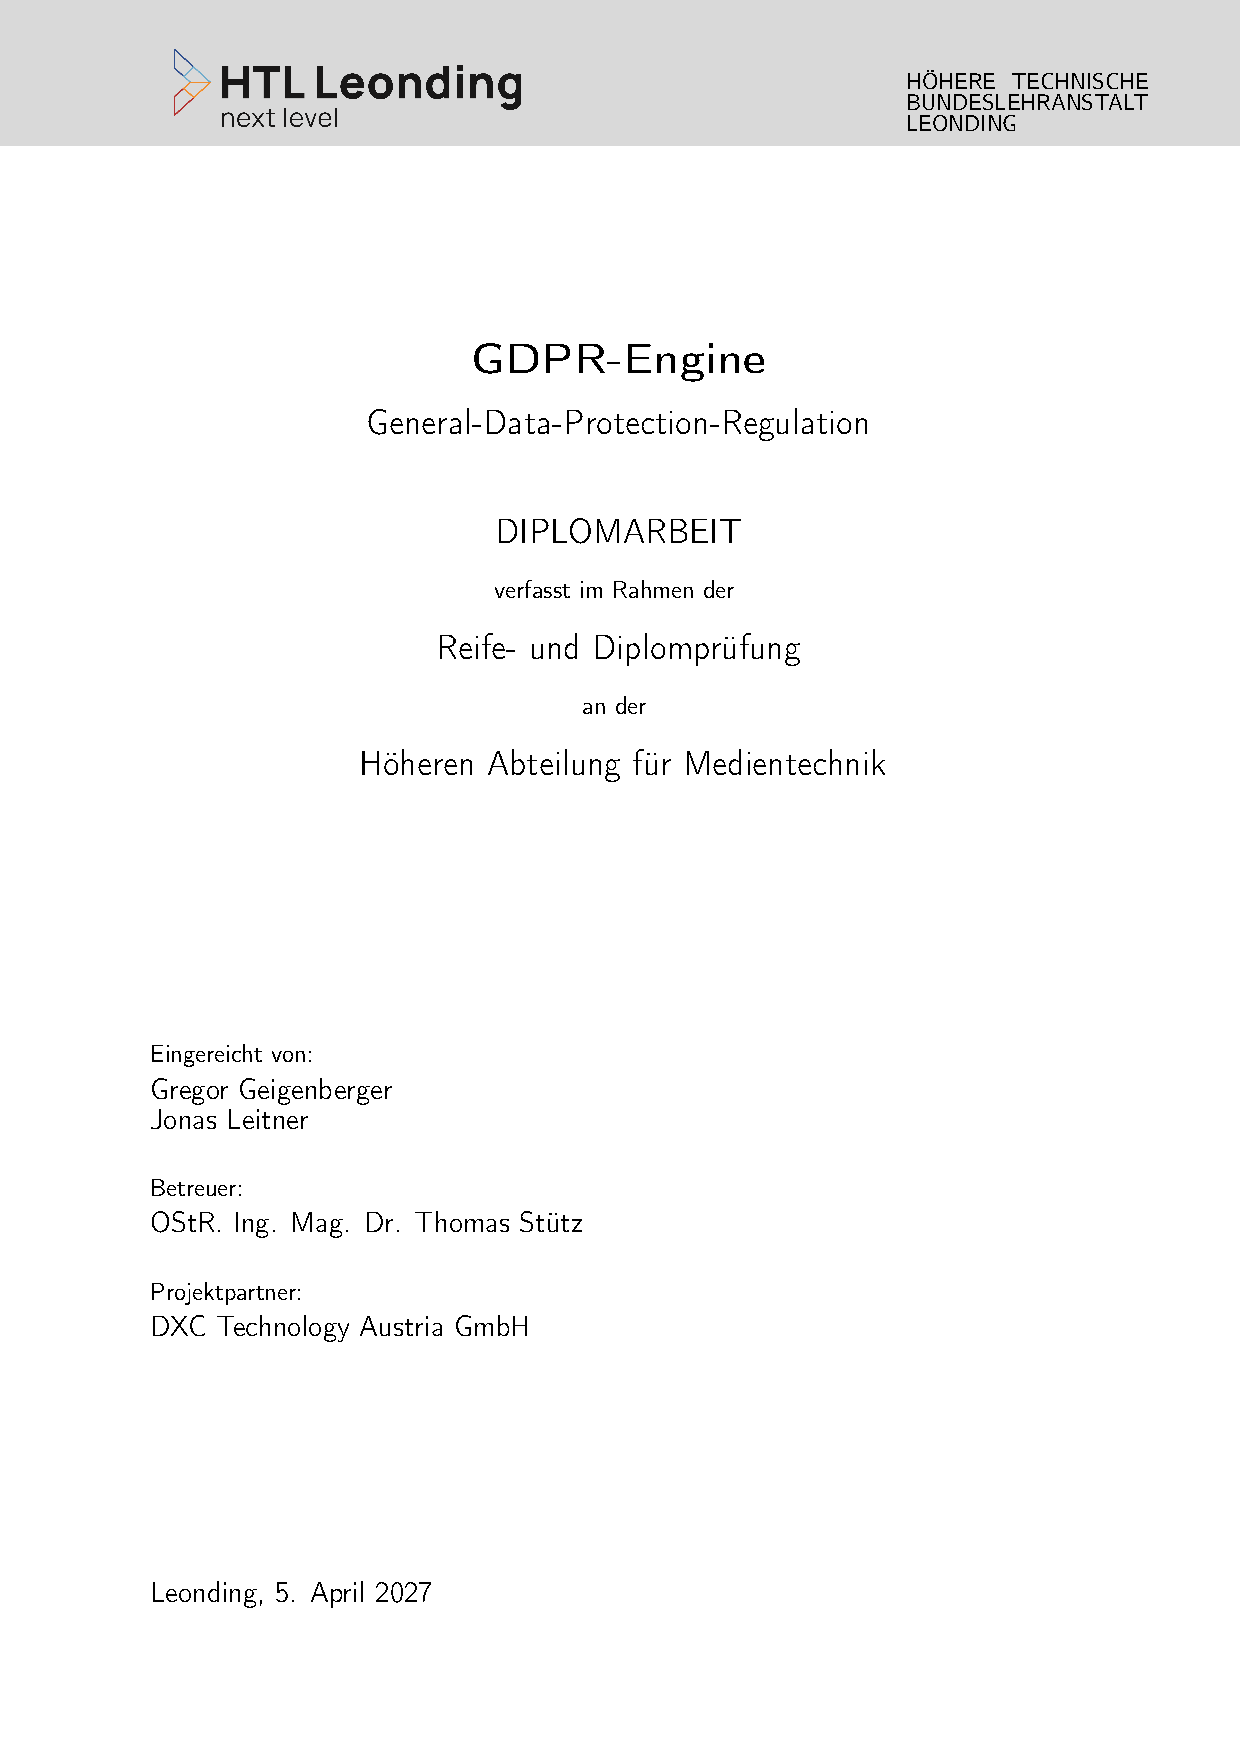
\includepdf{./titlepage/coversheet}
\pagenumbering{Roman}
\newpage
\input{oath}
% both abstracts are required, independent of the thesis language
\selectlanguage{english}
\begin{spacing}{1}
    \chapter*{Abstract}
\end{spacing}
\begin{wrapfigure}{r}{0.3\textwidth}
    \begin{center}
      \includegraphics[width=0.2\textwidth]{pics/question_mark.png}
    \end{center}
\end{wrapfigure}
Brief summary of our amazing work. In English.
This is the only time we have to include a picture within the text.
The picture should somehow represent your thesis.
This is untypical for scientific work but required by the powers that are.
\lipsum[6]
\newpage
\selectlanguage{ngerman}
\begin{spacing}{1}
    \chapter*{Zusammenfassung}
\end{spacing}
Die GDPR-Engine ermöglicht es für Kunden, ihre Daten, welche in vielen unterschiedlichen Microservices gespeichert sind, zu verwalten.
Hierbei haben die Kunden die Möglichkeit, ihre Daten zu verschlüsseln, entschlüsseln, anzuschauen oder zu anonymisieren.

Je nach Rolle des Kunden, greift die Engine auf unterschiedliche Microservices zu, um die Daten zu verwalten.
Hierbei ist wichtig, dass die Engine den Zugriff auf wichtige Daten, wie zum Beispiel Rechnungen nicht erlaubt,
da jene laut DSGVO nicht sofort gelöscht werden dürfen und später noch für die Buchhaltung benötigt werden.

Weiters werden sämtliche Zugriffe auf die Daten protokolliert und gespeichert, somit kann jederzeit
nachvollzogen werden, wer wann auf welche Daten zugegriffen hat oder jene verändert hat.

\emph{Bitte auf keinen Fall mit der Zusammenfassung verwechseln, die den Abschluss der Arbeit bildet!}
\langselect{\selectlanguage{ngerman}}{\selectlanguage{english}}

\input{glossary}

\pagestyle{plain}

\IfStrEq{\thesislang}{de}
{
	\renewcommand{\lstlistlistingname}{Quellcodeverzeichnis}
}
{
 % keep at list of listing
}

\tableofcontents
\newpage
\setcounter{RPages}{\value{page}}
\setcounter{page}{0}
\pagenumbering{arabic}
\pagestyle{scrheadings}

\begin{spacing}{1}
\chapter{\langselect{Einleitung}{Introduction}}\label{chapter:introduction} % fixed chapter
\end{spacing}
\input{./sections/introduction}

% content chapters: adapt, add or remove as needed
% use \langselect{German}{English} or simply write the title in the thesis language
\begin{spacing}{1}
\chapter{\langselect{Umfeldanalyse}{Related Work}}
\end{spacing}
\input{./sections/related_work}

\begin{spacing}{1}
\chapter{\langselect{Technologien}{Technologies}}\label{chapter:tech}
\end{spacing}
\input{./sections/technologies}

\begin{spacing}{1}
\chapter{\langselect{Umsetzung}{Implementation}}\label{chapter:implementation}
\end{spacing}
\input{./sections/implementation}

\begin{spacing}{1}
\chapter{\langselect{Zusammenfassung}{Summary}}\label{chapter:summary} % fixed chapter
\end{spacing}
\input{./sections/summary}

\newpage
\pagenumbering{Roman}
\setcounter{page}{\value{RPages}}
%\setlength{\glsdescwidth}{0.8\linewidth}
\glsnogroupskiptrue
\IfStrEq{\thesislang}{de}
{
	\printglossary[title=Glossar,toctitle=Glossar] %,style=long]
}
{
	\printglossary[title=Glossary,toctitle=Glossary] %,style=long]
}
\spacing{1}{
\IfStrEq{\thesislang}{de}
{
	\bibliographystyle{ieeetrande}
}
{
	\bibliographystyle{IEEEtran}
}
\bibliography{bib}
}
\listoffigures
\listoftables
\lstlistoflistings
\appendix
\addchap{\langselect{Anhang}{Appendix}}
\input{./sections/appendix}
\end{document}

